% REPLACE: "recall" instead of "factual" knowledge questions
% INTRO: motivate process/structure NOT content

% OUTLINE INTRO %
% 1. Assessing political competence is important, but the measurement debate remains unresolved
% 2. Factual knowledge questions are insufficient, we should focus on what people know and not what they don't know
% 3. This is where my measure comes in, describe basic idea and contribution
% 4. Outline of the paper and describe basic findings + conclusion

Political sophistication is one of the most fundamental concepts in the study of political attitudes and behavior---a crucial moderator impacting a range of mechanisms such as political decision-making and vote choice \citep{macdonald1995political,lau2001advantages}, persuasion and motivated reasoning \citep{zaller1992nature,lodge2013rationalizing}, or the susceptibility to misinformation \citep{vegetti2020impact}. Yet, fundamental issues regarding the measurement of political sophistication continue to plague the discipline \citep{mondak2001developing,sturgis2008experiment,bullock2021response}. Scholars usually rely on survey questions that assess people's ability to recall basic facts about political institutions and officeholders as a proxy for sophistication \citep{carpini1993measuring,barabas2014question}. In principle, these factual knowledge questions should cover information that is necessary for citizens to make competent decisions in a given context, but determining such a set of items proves to be extremely difficult \citep{lupia2006elitism}. Even within a given policy area, people may disagree about which facts are crucial for political competence due to inherent value differences \citep{lupia2015uninformed}. Furthermore, different sets of knowledge questions vary in difficulty across subgroups of the population, which can introduce systematic measurement error \citep{pietryka2013analysis}.

One manifestation of such systematic measurement error is the oft-cited gender gap in political sophistication. On the basis of conventional factual knowledge scores, women frequently appear to be less informed about politics than men \citep{verba1997knowing,wolak2011roots,fraile2014women}. To a certain extent, these findings may reflect genuine differences in political interest between men and women due to gendered socialization \citep{bos2021one}. However, at least part of the observed gender gap can be attributed to how we measure political knowledge. For instance, men tend to have a higher propensity to guess when answering recall questions, thus overestimating their knowledge levels \citep{mondak2004knowledge,fortin2020political}. Other research found that gender differences are attenuated when focusing on gender-relevant political knowledge \citep{dolan2011women}, by providing policy-specific information \citep{jerit2017revisiting}, or in contexts with more equitable representation of women \citep{pereira2019gendered}.

In this paper, I re-examine the gender gap by proposing a measure of \textit{discursive sophistication} that is based on how people discuss their political preferences in open-ended survey responses. Specifically, I develop a framework to assess whether beliefs and attitudes are expressed in a more elaborate manner---a question that is not directly discernible from off-the-shelf factual knowledge items. %The approach is therefore \textit{naive} in that it does not presuppose pieces of information as necessary for political competence but rather examines the respondents' justification of their preferences at face value. 
Measuring sophistication based on how people talk about politics provides two major advantages compared to off-the-shelf factual knowledge items: (1) it captures the extent to which a respondent's political beliefs are based on elaborate reasoning, and (2) it can easily pinpoint competence in specific areas by incorporating targeted open-ended items. The resulting measurement is therefore conceptually closer to the underlying latent trait of interest: the degree of structure and constraint in political belief systems \citep{tetlock1983cognitive,luskin1987measuring}. Furthermore, it can be easily applied by researchers interested in analyzing open-ended responses with an easy-to-use software package available in the statistical programming environment R.\footnote{Package under development, release on CRAN expected mid 2022.}

I validate the measure across multiple representative surveys in the United States and Europe encompassing four languages (total $N \simeq 35,000$) by comparing it to conventional factual knowledge scores as predictors of various indicators of civic competence and engagement. While discursive sophistication shares a considerable amount of variance with traditional metrics, they are far from equivalent. Indeed, discursive sophistication is a stronger predictor of turnout and other forms of political engagement. Contrary to previous research, however, I find no evidence for a gender gap in discursive sophistication. While women might score lower than men on factual knowledge about political institutions and elites, there are no differences in the complexity of expressed political attitudes. Furthermore, I present suggestive evidence that this divergence can be explained by the fact that open-ended responses allow women to focus on different issues than men. In sum, the results suggest that exploring open-ended responses provides new opportunities to examine political sophistication across time and contexts.


\section*{Political Sophistication and Factual Knowledge}

% OUTLINE THEORY %
% 1. Everyone uses knowledge, and it's usually off-the-shelf stuff
% 2. Since it's infeasible to come up with new knowledge battery for every problem, Druckman argues that we should focus on the process rather than the content/substance
% 3. Previous researchers have induced in-depth processing by asking people to justify their preferences
% 4. I ask the question of how people should justify their preferences if they engage in in-depth processing! 
% 5. Examining how people justify their preferences is also important because that's how social infleunce etc. is transmitted.
% 6. (optional) Segway to discuss how these attributes of elaborate processing and sophisticated belief systems should be expressed in open-ended responses.

% Many studies use factual knowledge as a proxy for sophistication
Public opinion researchers routinely incorporate political sophistication in their empirical analysis in one way or another---either directly as an outcome variable of interest, as a major explanatory factor, or as an important confounder to control for. In order to measure the underlying latent trait, scholars commonly rely on short batteries of standard recall questions on basic facts about the political system.\footnote{For example, the American National Election Study routinely asks questions such as, ``Do you happen to know which party currently has the most members in the U.S. Senate?''} One canonical article proposing such a battery---\citet{carpini1993measuring}---has been cited more than 1000 times since its publication. Figure~\ref{fig:carpini} shows the yearly citation count over time; the trend illustrates how political knowledge remains a concept of intense scholarly interest---and that it is frequently measured using standard off-the-shelf recall questions.

\begin{figure}[h]\centering
	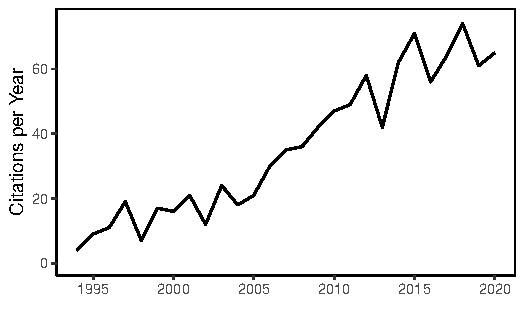
\includegraphics{/data/Dropbox/Uni/projects/2016/knowledge/fig/cites.pdf}
	\caption[Yearly citation count of \citet{carpini1993measuring}]{Yearly citation count of \citet{carpini1993measuring} based on Google Scholar.}\label{fig:carpini}
\end{figure}

% Low levels of political sophistication
The ubiquity of basic recall questions in public opinion research is accompanied by the frequent finding that many people know too little about politics \citep{carpini1996americans,barabas2014question} and the discrepancies in information levels can result in unequal representation in the political system \citep{althaus1998information,kuklinski2000misinformation,gilens2001political}. The underlying reason why scholars focus on people's ability to recall factual information about politics is that these items ``more directly than any of the alternative measures, capture what has actually gotten into peoples minds'' (\citealt[21]{zaller1992nature}; see also \citealt{zaller1991information,gomez2001political}). However, there is some reason to doubt this assertion, both from theoretical as well as methodological perspectives.

% Conceptual criticism
First, the discipline's focus solely on factual political knowledge has been criticized on theoretical grounds. Most importantly, recalling facts about political institutions  has little relevance for citizen competence \citep{lupia2006elitism,cramer2017fact}. Given that there is usually no consensus about what information is necessary in the first place, \citet{druckman2014pathologies} proposes abandoning recall questions as measures of ``quality opinion.'' Instead, the author advocates ``\textit{less} focus on the \textit{content/substance} of opinions [...] and \textit{more} on the \textit{process} and specifically the \textit{motivation} that underlies the formation of those opinions'' \citeyearpar[478, emphasis in the original]{druckman2014pathologies}. The key distinction should therefore be how citizens approach a political issue and whether they are motivated to engage in elaborate reasoning to arrive at their particular decision. In addition, researchers should concentrate on heuristics that directly help citizens to make competent political decisions or focus only on knowledge relevant to a specific task \citep[see also][]{lupia1994shortcuts}. Accordingly, there is no need for individuals to know all available facts, but only to possess the skills and resources to be able to find the information required in a specific context \citep{prior2008money}. Furthermore, conventional items differ with regard to the dimension of political knowledge they measure \citep{barabas2014question} and ignore important aspects such as visual cues \citep{prior2014visual}.

% Methodological criticism
Second, there are several methodological issues that cast doubt on the validity of factual knowledge scores as a measure of political sophistication. One problem frequently discussed in the literature centers around the question whether or not to offer ``Don't Know'' options in multiple choice recall questions \citep{mondak2000reconsidering,mondak2001asked,miller2008experimenting}. Including such an option can lead to biased estimates of information levels because they are confounded by people's differential propensity to guess instead of admitting not to know the correct answer \citep[but see][]{luskin2011don}. Other scholars criticized open-ended factual knowledge questions due to problematic coding rules, which do not capture partial knowledge \citep{krosnick2008problems,gibson2009knowing,debell2013harder}. The increasing reliance on online surveys instead of phone or face-to-face surveys creates additional concerns due to people's (differential) tendency to cheat by looking up answers for recall questions \citep{clifford2016cheating,hohne2021looking,style2021does}. Lastly, factual knowledge scores have been shown to suffer from differential item functioning, since individual recall questions have varying measurement properties across the population \citep{pietryka2013analysis}. Item batteries that are easier to answer for certain groups can therefore exacerbate observed differences in political knowledge---for example between racial groups \citep{abrajano2014reexamining}.


\section*{Please Mind the Gender Gap}

Survey researchers not only find that people are not sufficiently informed as a whole, they also attest that women are systematically less knowledgeable than men. For instance, \citet{verba1997knowing} report that women score lower on political information, interest, and efficacy, which decreases their respective levels of political participation. Since gender differences in political information and interest can only partly be explained by resource-related factors such as individual levels of education, the authors diagnose a ``genuine difference in the taste for politics'' between women and men, which they suspect is driven largely by socialization \citep[see also][]{wolak2011roots}. Indeed, \citet[117]{dow2009gender} describes the systematic gender differences in knowledge as ``one of the most robust findings in the study of political behavior.'' While differences between women and men in political \textit{interest} can certainly be attributed to gendered political socialization \citep{bos2021one,wolak2020self}, at least part of the disparities in \textit{knowledge} may simply be an artifact of the measurement approach.

The discussion revolving around the apparent gender gap is therefore closely intertwined with the methodological debate about measuring political knowledge. For instance, \citet{mondak2004knowledge} suggest that women are more likely to report that they do not know the answer to a recall question whereas men are more inclined to guess. Correcting for the systematic differences in the propensity to guess, however, mitigates the gender gap in knowledge but does not eliminate it completely \citep[see also][]{lizotte2009explaining,ferrin2017gender}. Other aspects of the survey context have been shown to affect gender differences in political knowledge as well. \citet{mcglone2006stereotype} present evidence that the gender gap is exacerbated in an environment that induces stereotype threat, such as if women are aware of the fact that the study focuses on gender differences or if they are interviewed by a male interviewer. However, gender differences are not only induced by \textit{how} researchers ask their questions, but also by the question \textit{content}. Focusing on gender-relevant political knowledge items such as information about women's representation in the federal government has been shown to close the gap \citep{graber2001processing,dolan2011women,fraile2014does,jerit2017revisiting}. Similarly, the gender gap is reduced or disappears when people are asked about more practical issues related to the government such as the availability of benefits and services \citep{stolle2010women}, or in political contexts characterized by more equitable representation of women \citep{pereira2019gendered,mcallister2019gender,wolak2019descriptive}. Importantly, women's lower factual knowledge score does not appear to impede on their political competence. In fact, \citet{dassonneville2020women} find that women are no less likely to vote for candidates who represent their preferences, and are therefore able to participate in politics just as effectively as men.

Overall, the gender gap appears to be influenced by how we ask for political information in surveys, as well as the kind of knowledge that is required for a correct response. Indeed, a comprehensive cross-national analysis of election studies in 47 countries between 1996 and 2011 suggests that question format and content account for large portions of the variance of gender disparities in political knowledge \citep{fortin2016cross,fortin2020political}. In short, conventional knowledge measures have problematic measurement properties that may exacerbate observed gender differences. 


\section*{Back to the Roots: The Structure of Belief Systems}
% Attitude Expression and Elaborate Reasoning
% Conceptualizing Discursive Sophistication

% OUTLINE MEASUREMENT %
% 1. How can we characterize in-depth processing in open-ended responses? We don't want to look at textual complexity, as other recent research has done.
% 2. It's about the speaker, not the recipient! This is were the literature on belief systems comes in! Theoretical accounts of political sophistication as the basis for elaborate and in-depth political reasoning
% 3. Derive the three dimensions conceptually, connect them to belief system literature -> survey example!
% 4.-6. Now we discuss how we can measure them in open-ended responses

% How can we characterize the level of sophistication in open-ended responses that engage in more in-dpeth processing? This is where the literature on belief systems comes in.
% Next, I will explore specific attributes that allow us to distinguish more or less elaborate reasoning in open-ended responses.
% If we To the extent that people's political sophistication and competence manifests itself in attitude expression 
% Recent studies in political science, for example, used measures based on the readability or comprehensibility to study the sophistication of political communication
% measuring the degree of elaborate reasoning in verbatim attitude expression

% Factual knowledge about is all but a proxy for an underlying latent trait: political sophistication. 
Despite the discipline's reliance on off-the-shelf item batteries, factual knowledge about political institutions has little overlap with the requirements for political competence---leading some scholars to suggest that we should abandon recall questions as measures of ``quality opinion'' \citep{druckman2014pathologies}. From a theoretical perspective, knowledge scores are all but a proxy for an underlying latent trait---political sophistication---which is usually conceptualized based on people's belief systems instead of focusing on isolated pieces of factual information stored in declarative memory. Belief systems are defined as ``a configuration of ideas and attitudes in which the elements are bound together by some form of constraint or functional interdependence'' \citep[207]{converse1964nature}.

Political sophistication can then be characterized by how these ideas and attitudes (or considerations) are structured along three different dimensions \citep{luskin1987measuring}. The first, and most obvious one, is the \textit{size} of a belief system, which simply describes the number of distinct considerations that are available for retrieval. Politics, however, is comprised of a diverse set of independent domains---with some people having a deep grasp of a narrow field and others having a broad and potentially more shallow understanding of various issues. Thus, the second dimension describes the \textit{range} of a belief system across domains (e.g,. different policy issues or other evaluative categories). The last dimension is a belief system's \textit{constraint}, which describes the extent to which considerations are organized in a meaningful way through differentiation and integration of competing cognitions \citep{luskin1987measuring}. In other words, this dimension captures whether available considerations are perceived as operating in isolation or are rather as part of a more complex interconnected system, for example by identifying inherent value conflicts \citep{tetlock1983cognitive,tetlock1993cognitive}. To summarize, I conceptualize political sophistication based on the \textit{structure} of individual belief systems along the following three dimensions:

\begin{enumerate}
	\item \textbf{Size:} \textit{The number of considerations associated with a given category or issue.}
	\item \textbf{Range:} \textit{The dispersion of considerations across different categories or issues.}
	\item \textbf{Constraint:} \textit{The extent to which considerations are interconnected in a meaningful way.}
\end{enumerate}

Political sophistication, in turn, is the conjunction of these dimensions: ``A person is politically sophisticated to the extent to which his or her [political belief system] is large, wide-ranging, and highly constrained'' \citep[860]{luskin1987measuring}. Similarly, \citet{tetlock1983cognitive,tetlock1993cognitive} coined the term \textsl{integrative complexity} to describe the degree to which considerations related to an issue are interconnected. In short, sophisticated political reasoning should reflect this notion of complex belief systems.\footnote{It should be no surprise that Converse and others examined open-ended responses in their early studies--albeit from a slightly different perspective than the approach outlined here. Importantly, instead of relying on manual coding of open-ended responses, I develop an automated framework that is easily reproducible and can directly be applied to large surveys.}

% TODO: more on contraints


\section*{Measuring Discursive Sophistication}
% A First Look at Discursive Sophistication

% Rather than trying to develop recall items that presupposes a set of facts as necessary for political competence, I therefore analyze \textit{how} individuals discuss their preferences related to a given political task.

% Of course, we cannot measure the structure of belief systems directly, but we can examine observable implications.
Given that recall questions are only an imperfect measure for political sophistication, it is worth considering alternative---and potentially more imminent---observable implications of the underlying latent trait of interest: complex and highly constrained political belief systems. In the following, I propose a framework that leverages the content of open-ended responses in conjunction with the survey structure to evaluate how people discuss their political beliefs and preferences in their own words. To illustrate the approach in the context of a concrete example, consider a questionnaire where respondents is prompted to answer the following open-ended prompt:
% In developing a measure of political sophistication, we are ultimately interested in the structure of people's belief system.

\begin{quote}
	On the issue of \textbf{gun legislation}, please outline the main arguments that come to mind \textit{in favor and against} background checks for all gun sales, including at gun shows and over the Internet.
\end{quote}

Now suppose that this questionnaire includes a whole set of similar items on other topics such as \textbf{abortion}, \textbf{immigration}, \textbf{health cure}, and \textbf{trade policies}---each asking respondents for both positive or negative considerations related to specific policy proposals. How would a complex and constrained set of political beliefs manifest itself across such a battery of open-ended responses? I argue that each dimension outlined above has direct observable implications for individual response behavior.

First, the \textit{size} of a belief system is defined as the number of available considerations associated with a given category or issue. In the context of open-ended survey questions, a large belief system should therefore allow people to discuss their views by raising a larger number of distinct topics in response to each query. While this could also be achieved through manual coding, I rely on the structural topic model framework to extract the number of topics mentioned by each respondent in a survey \citep{roberts2014structural}.\footnote{Please refer to the appendix for additional information. Specifically, see Appendix~\ref{app:oeinfo} for descriptive information on open-ended responses in each data set and structural topic model results. Appendix~\ref{app:topicmodel} contains further details on pre-processing steps and modeling choices for the structural topic models as well as robustness checks, which include preText analyses proposed by \citet{denny2018text}.} Let $\mathcal{W}_i$ denote the set of words contained in a response of individual $i$. Each word $w\in\mathcal{W}_i$ is assigned to a topic $t^* \in \{1,...,T\} $, such that $P(t^*|w,X_i) > P(t|w,X_i) \forall t\neq t^*$.\footnote{Note that $P(t|w,X_i)=\tfrac{P(w|t)P(t|X_i)}{P(w|X_i)}$. In the context of structural topic models, $X_i$ denotes the covariates used to predict individual topic prevalence \citep[see][for details]{roberts2014structural}. I used measures for age, gender, education, party identification, as well as an interaction between education and party identification as covariates for topic prevalence. This variable selection---with the exception of including gender---is equivalent to the procedure described in \citet{roberts2014structural}.} In other words, each unique term in a response is assigned to the topic that has the highest likelihood of having generated that term, given the model. The set of topics that are mentioned by respondent $i$ across all words in $\mathcal{W}_i$ can then be described as $\mathcal{T}^*_i$ and the number of considerations can be written as:
\begin{equation}
\text{size}_i = \dfrac{|\mathcal{T}^*_i|}{\max|\mathcal{T}^*_i|}.
\end{equation}
I re-scale the measure to range from zero to one by dividing raw count of topics by the maximum number of topics observed across individuals.

Second, the \textit{range} of a belief system is defined as the dispersion of considerations across categories or issues. Given a set of survey prompts covering various political issues, high levels of sophistication should correspond with people's ability to respond to each query with comparable levels of elaboration. I therefore quantify the consistency in response behavior across items by computing the Shannon entropy in open-ended response lengths:
\begin{equation}
\text{range}_i = \dfrac{-\sum_{j=1}^J p_{ij} \ln p_{ij}}{\ln J}
\end{equation}
where $p_{ij}$ is the proportion of words in the response of individual $i$ to question $j\in \{1,...,J\}$ relative to the overall size of the individuals' response. The variable ranges from 0 (only one question was answered) to 1 (all questions were answered with the same word length per answer).

The last component addresses the level of \textit{constraint} between considerations. The extent to which considerations are interconnected in a meaningful way should be associated with people's ability to differentiate and/or integrate them in their reasoning \citep{tetlock1993cognitive}. Following \citet{tausczik2010psychological}, I rely on specific function words as linguistic markers for these processes. More specifically, differentiating competing considerations in speech is usually accomplished using exclusive words (e.g., but, without), while integrating multiple thoughts is accomplished by the use of conjunctions (e.g., and, also). Thus, I measure relative constraint by identifying the number of conjunctions ($\text{CONJ}_i$) and exclusive words ($\text{EXCL}_i$) in each open-ended response using the Linguistic Inquiry and Word Count (LIWC) dictionary \citep{pennebaker2015development}:
\begin{equation}
\text{constraint}_i = \dfrac{\text{CONJ}_i + \text{EXCL}_i}{\max\left[\text{CONJ}_i + \text{EXCL}_i\right]}
\end{equation}
As before, I re-scale the measure to range from zero to one by dividing all values by the empirical maximum observed across all individuals in the data.

Together, the three measures can be combined in a composite metric of sophistication in political attitude expression by averaging them for each respondent. Like each individual component, the resulting \textit{discursive sophistication} score ranges from 0 to 1:
\begin{equation}
\text{discursive sophistication}_i = \tfrac{1}{3}(\text{size}_i + \text{range}_i + \text{constraint}_i).
\end{equation}

% Discursive sophistication in attitude expression is then defined as the conjunction of these three basic dimensions.
%In a questionnaire where respondents are asked to discuss their political attitudes in multiple open-ended items, I therefore define discursive sophistication as the conjunction of the three dimensions described here. 
Overall, a highly sophisticated individual should therefore give a more \textit{elaborate} response across the full \textit{range} of questions by \textit{integrating} and/or \textit{differentiating} multiple considerations. Note that this simple framework makes no assumptions about the direction of people's attitudes or their specific ideology. Crucially, since it is solely based on \textit{how} individuals discuss their preferences, it can be directly applied in various settings to target specific political issues or tasks such as choosing between candidates running for election.
% In the following, I discuss these three different attributes of open-ended survey responses that should be indicative of sophistication in attitude expression in more detail.

Of course, this is not the first time a framework is developed to assess the complexity of written (or spoken) word. In fact, this task has been the subject of longstanding research in linguistics and educational sciences, resulting in a multitude of alternative metrics. Recently, these measures have been employed by political scientists who study different forms of elite communication. \citet{spirling2016democratization}, for example, uses a standard readability score based on the ratio of words per sentence and syllables per word to study the linguistic complexity of speeches in the British House of Commons over time. More recently, \citet{benoit2019measuring} expanded on previous metrics to develop a measure of comprehensibility that is more applicable in the realm of politics.
% \citet{spirling2016democratization}: The findings reveal that ministers started to use simple language in the parliament after suffrage was expanded in the middle nineteenth century---presumably in an effort to appeal to the enlarged voter base. 

These approaches---and especially the development of metrics specifically suited for political text---are particularly useful when studying elite communication. Yet, in contrast to the framework outlined above, they focus on the \textit{comprehensibility} as a measure of complexity; elite sophistication is evaluated based on a recipient's ease to understand the message, which is largely driven by linguistic and syntactic difficulty rather than actual political content. While this is certainly a reasonable approach when studying the effects of elite communication, the inference of interest outlined in this paper is markedly different. My focus is to examine verbatim attitude expression to assess the underlying degree of elaborate political reasoning. Pure linguistic style is therefore not of central concern so long as it is unrelated to the actual political content.\footnote{In fact, pure linguistic complexity is arguably driven more by other factors such as a person's general verbosity or linguistic prowess and therefore less valid as a measure of political sophistication.} After all, being hard to comprehend does not necessarily imply that someone put a lot of thought into a statement.
% Reading level measures essentially focus on how hard it is to understand the author. This makes sense if we are primarily interested in the messaging aspect, for example when analyzing speeches of political elites. When it comes to individual levels of sophistication, a pure focus on linguistic patterns are less ideal.
% However, while these techniques are certainly useful to examine complexity in messaging by political elites, they may be highly confounded by personal verbosity and linguistic prowess. Instead of assessing linguistic style, we want to target the complexity in the actual content. Rather than measuring how a specific attitude is delivered, we want to focus on the the complexity in what is being said.
% The inference of interest is not how easy it is to understand someone, but rather how much thought went into what has been said. Both are clearly correlated, but they should not be assumed to be equivalent.
% comprehensibility of the text captures more of the linguistic ability independent of the underlying political content.

% TODO: add argument here regarding biases in manual coding.


\section*{Results}

To evaluate my proposed measure of discursive sophistication, I included the battery of open-ended questions described above in a 2018 wave of the Cooperative Election Study (CES),\footnote{Formerly Cooperative Congressional Election Study (CCES).} which consists of a national stratified sample of 1,000 respondents. In addition, I illustrate the versatility and robustness of the approach by applying the measure across multiple previously collected surveys that employ a range of alternative open-ended items. Below is a summary of all data sets and items used in the subsequent analysis:\footnote{A detailed description of each data set and the specific question wording is included in Appendix~\ref{app:variables}.}

\begin{itemize}\singlespacing
	\item \textbf{Cooperative Election Study (CES 2018):} 10 open-ended questions targeting policy preferences on gun legislation, abortion, immigration, health care, and trade.
	\item \textbf{American National Election Study (ANES 2020, 2016, 2012):} 8 open-ended likes-dislikes questions targeting preferences for parties and candidates.
	\item \textbf{YouGov Survey (2015)}: 4 open-ended questions targeting policy preferences on gun legislation and health care.
	\item \textbf{Swiss Referendum Surveys (2012-2008)}: 2 open-ended questions asking respondents to justify their vote choice in various policy referenda. These surveys were conducted in three languages (French, German, and Italian).
\end{itemize}

% Each survey focuses on sophistication in the context of distinct political tasks, namely the evaluation of (1) candidates running for public office, (2) broad issue areas such as health care and gun legislation, and (3) specific legislative policy referenda. The data sets are briefly described below.

I proceed by providing descriptive evidence regarding the face validity of discursive sophistication. Next, I assess its construct validity by comparing it to factual knowledge as a predictor of various relevant outcomes such as political participation and engagement. The last validation step consists of comparing discursive sophistication to manually coded levels of justification in open-ended responses. Each of these steps leverage different subsets of the studies listed above, depending on the availability of necessary items. After validating the measure, I assess gender gaps in discursive sophistication and factual knowledge using the complete set of surveys.


\subsection*{A First Look at Discursive Sophistication}

While each dimension of discursive sophistication outlined above provides a unique source of variance to the underlying concept \citep{luskin1987measuring}, all three are positively correlated.\footnote{See Appendix~\ref{app:oeinfo} for correlation matrices between individual components.} Furthermore, exploratory factor analyses confirm that they load on a single factor with all loadings exceeding 0.5 across the CES and ANES data---thus confirming that we can rely on an additive score to measure discursive sophistication (see Table~\ref{app:factload}).\footnote{I rely on the CES and ANES here since these surveys employ a larger set of open-ended questions.}

% latex table generated in R 4.2.1 by xtable 1.8-4 package
% Wed Aug 10 12:57:08 2022
\begin{table}[ht]
\centering
\begin{tabular}{lcccc}
  \hline
Variable & 2018 CES & 2020 ANES & 2016 ANES & 2012 ANES \\ 
  \hline
Size & 0.840 & 0.997 & 0.997 & 0.997 \\ 
  Range & 0.526 & 0.536 & 0.548 & 0.576 \\ 
  Constraint & 0.513 & 0.684 & 0.623 & 0.709 \\ 
   \hline
\end{tabular}
\caption{Factor Loadings of Discursive Sophistication Components} 
\label{app:factload}
\end{table}


How does this discursive sophistication score compare to alternative metrics of political knowledge? As discussed, the standard approach to measuring political knowledge in surveys is to ask a set of factual questions about political institutions. The CES and ANES include such a basic item battery, inquiring for example about presidential term limits or the majority party in either chamber of Congress. I combine responses on these items to form an additive index of \textit{factual knowledge} about politics. As an additional benchmark, I consider \textit{interviewer assessments} of each respondent's political sophistication (see \citealt{bartels2005homer}; but cf. \citealt{ryan2011accuracy}).\footnote{Interviewer assessments were only recorded in the face-to-face sample of the 2012 and 2016 ANES.}

\begin{figure*}[ht]
    \centering
    \begin{subfigure}[t]{0.45\textwidth}
    	\centering
    	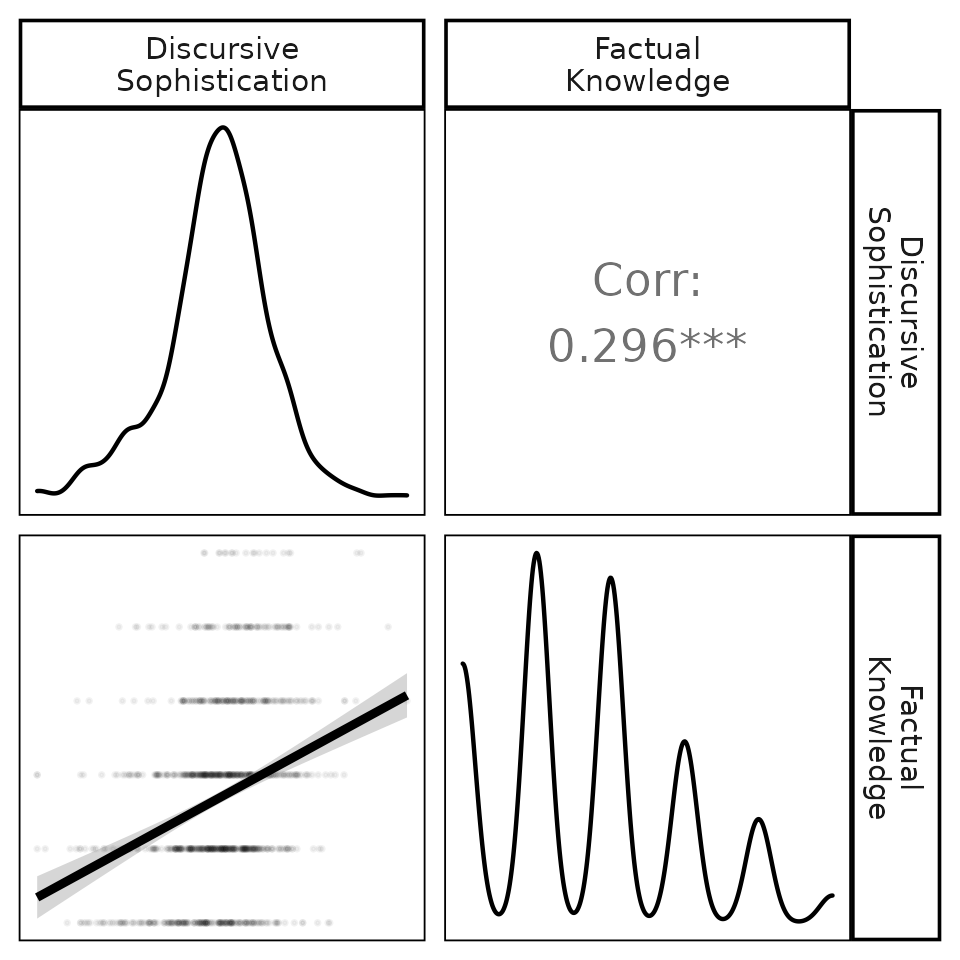
\includegraphics[scale=.7]{/data/Dropbox/Uni/projects/2016/knowledge/fig/cces2018_corplot.png}
    	\caption{2018 CES}
    \end{subfigure}
	~~
    \begin{subfigure}[t]{0.45\textwidth}
    	\centering
    	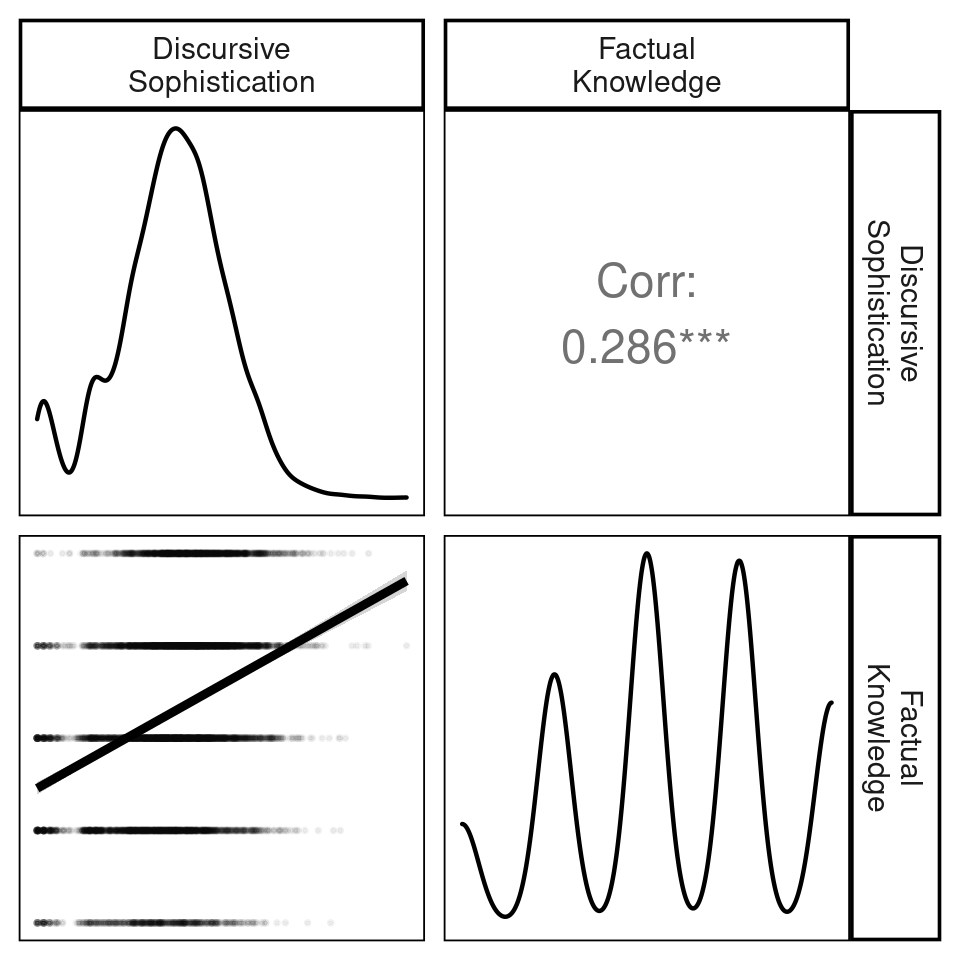
\includegraphics[scale=.7]{/data/Dropbox/Uni/projects/2016/knowledge/fig/anes2020_corplot.png}
    	\caption{2020 ANES}
    \end{subfigure}
    \begin{subfigure}[t]{0.45\textwidth}
    	\centering
    	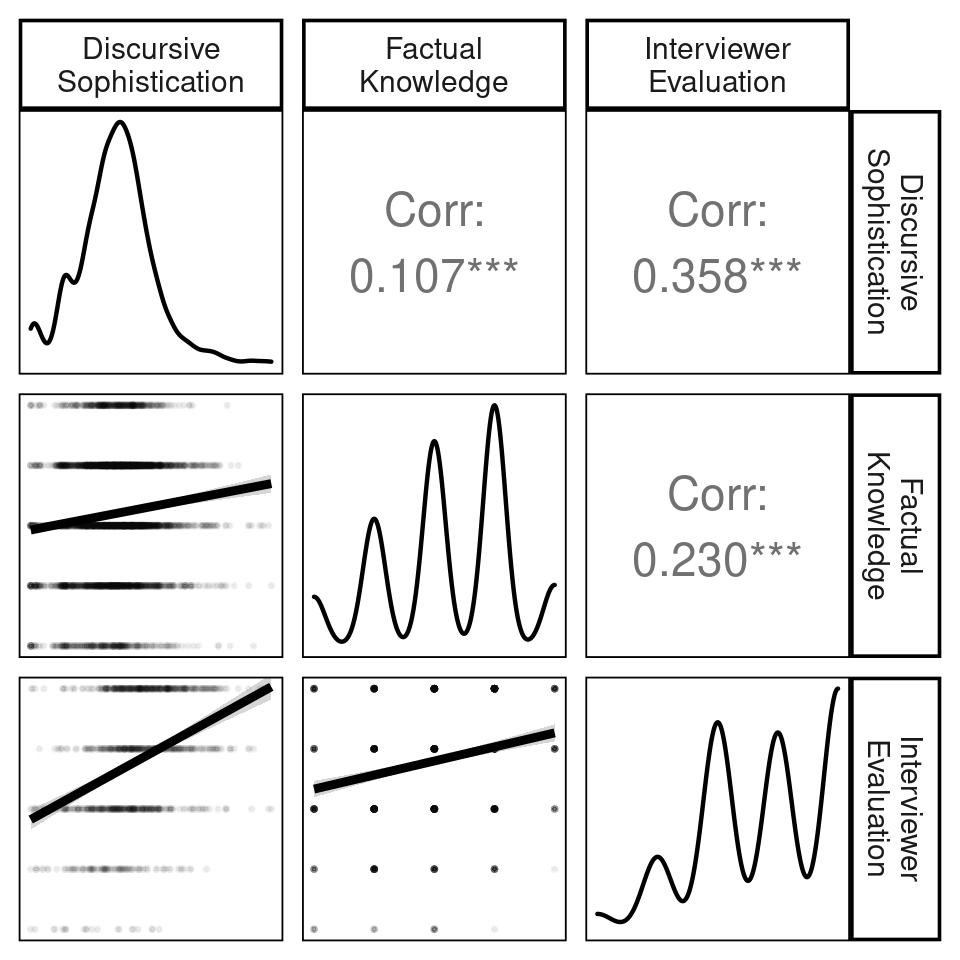
\includegraphics[scale=.7]{/data/Dropbox/Uni/projects/2016/knowledge/fig/anes2016_corplot.png}
    	\caption{2016 ANES}
    \end{subfigure}
	~~
    \begin{subfigure}[t]{0.45\textwidth}
        \centering
        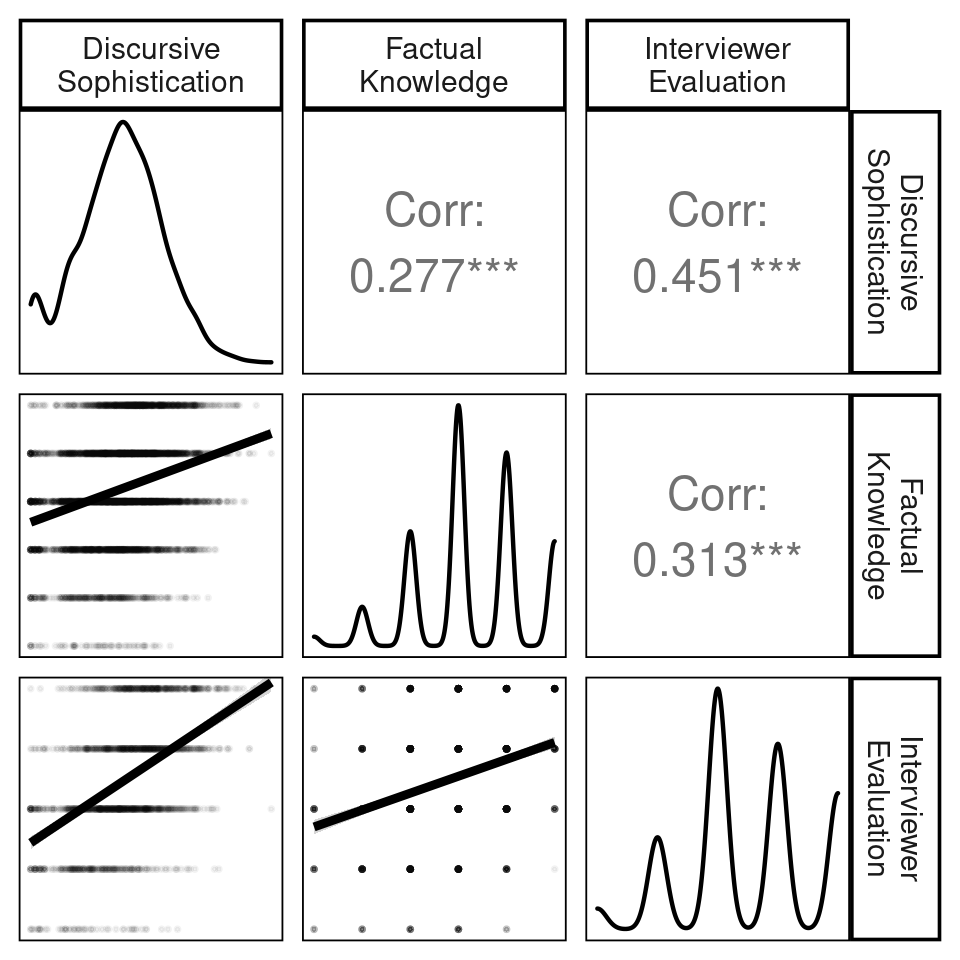
\includegraphics[scale=.7]{/data/Dropbox/Uni/projects/2016/knowledge/fig/anes2012_corplot.png}
        \caption{2012 ANES}
    \end{subfigure}%
    \caption[Correlation matrix of discursive sophistication and conventional political knowledge metrics]{Correlation matrix of discursive sophistication and conventional political knowledge metrics. The plots on the diagonal display univariate densities for each variable. The panels in the lower triangular display the scatter plot of two measures as well as a linear fit. The upper triangular displays the correlation coefficient. All correlations reported are statistically significant with $p<.05$.}\label{fig:corplot}
\end{figure*}

Figure~\ref{fig:corplot} compares discursive sophistication to the conventional knowledge metrics for the CES and ANES. Each figure presents scatterplots between individual measures (lower triangular), univariate densities (diagonal), and correlation coefficients (upper triangular). The measure of discursive sophistication is positively correlated with both conventional metrics while capturing some additional variation. Interestingly, there is a stronger correlation between discursive sophistication and interviewer evaluations than between factual knowledge and interviewer evaluations ($r=.36$ vs. $r=.23$ in 2016, and $r=.45$ vs. $r=.31$ in 2012), which indicates that the open-ended measure captures characteristics that influence subjective assessments of sophistication. Thus, a respondent's verbatim answers seem to be more influential for subsequent knowledge assessments by the interviewer than a respondent's performance on the factual knowledge questions.

While discursive sophistication and the alternative measures are clearly correlated, the relationship between each metric is far from perfect. To provide some intuition as to whether the variation in discursive sophistication is theoretically meaningful, I present an example of open-ended responses from two individuals in the 2018 CES who \textit{scored equally on factual knowledge} (3 out of 3 correct responses), but varied in discursive sophistication. 

\begin{table}[ht]\footnotesize\centering
\begin{tabular}{l|p{6.8cm}|p{5.8cm}}
\toprule
					& A: Low Sophistication Response 
					& B: High Sophistication Response
					\\\midrule
Guns (+)			& Increases the fact that bad actors will be caught before getting guns to cause problems
					& Making sure healthy law abiding citizens only can get guns
					\\\hdashline
Guns (-)			& Can't think of any
					& The second amendment....
					\\\hdashline
Abortion (+)		& Don't know
					& Killing babies
					\\\hdashline
Abortion (-)		& Don't know
					& Women want the right to decide what to do medically with their own bodies
					\\\hdashline
Immigration (+)		& It was not their fault they were brought here. If they are not committing crimes, they should be given a chance at citizenship
					& They have been living here for years and should not have to be uprooted
					\\\hdashline
Immigration (-)		& don't know
					& They came here illegally and are criminals
					\\\hdashline
Health care (+)		& It is too expensive - it requires people who don't use insurance or haven't in the pas to pay for everybody who does, especially the people who are getting it for free.
					& Cost to much, hurts the middle class, raised costs of health insurance
					\\\hdashline
Health care (-)		& Can't think of a thing.
					& Many people who get insurance through the ACA would be left uninsured
					\\\hdashline
Trade policy (-)	& don't know
					& More money for the government without taxing the people
					\\\hdashline
Trade policy (+)	& don't know
					& They are affecting trade relations, making products brought into the us more expensive
					\\\midrule
Disc. Soph. 		& 0.289
					& 0.517 
					\\\bottomrule
\end{tabular}
\caption[Example of open-ended responses for low and high scores on discursive sophistication]{Example of open-ended responses for low and high scores on discursive sophistication with equal factual knowledge scores (3 out of 3 correct responses). Column A displays the verbatim responses of an individual who scored low on discursive sophistication and column B displays the verbatim responses of an individual who scored high on the open-ended measure. Each row represents one of the likes/dislikes items included in the analysis. Note that the entries are original responses without editing.}\label{tab:ex1}
\end{table}

The results are presented in Table~\ref{tab:ex1}. Each row represents one of the open-ended responses targeting specific policy issues. Column A displays the responses of an individual who scored low on discursive sophistication and column B displays the responses of a high scoring individual. Even though both individuals have the same factual knowledge score, there are systematic differences in their response behavior that suggest disparity in their political sophistication. Overall, respondent A provided a less elaborate response and only focused on a narrow range of issues. Irrespective of whether one agrees with the specific statements, A's response pattern is suggestive of a less sophisticated political belief system and a lower level of motivation to engage in in-depth reasoning about each issue. Overall, this initial result suggests that the variation in discursive sophistication captures meaningful differences in response behavior that overlaps with traditional knowledge metrics while displaying some unique variation. The following sections will show that this variation is also politically consequential.

% TODO: Discuss how the high sophistication response elaborates more on effects of trade policy.



\subsection*{Validating the Measure}
% Discursive Sophistication and Political Competence

A crucial step in validating any measure of political sophistication is to examine the extent to which it is correlated with political engagement and citizen competence \citep{lupia2006elitism,lupia2015uninformed}. Accordingly, I consider how discursive sophistication is associated with (1) engagement and participation in politics, (2) the ability to incorporate new information, and (3) well-justified policy preferences.
% (5) vote choices that are consistent with underlying interests


\subsubsection*{Engagement and Participation in Politics}
Any measure of political sophistication should be strongly associated with individual engagement and participation in politics. In fact, factual knowledge items have been validated in the past based on their strong relationship with outcomes such as turnout and other forms of participation \citep[230--233]{lupia2015uninformed}. Figure~\ref{fig:knoweff} compares the effect of discursive sophistication and factual knowledge on four dependent variables related to political engagement: turnout, political interest, internal efficacy, and external efficacy. The model predicting turnout is estimated via logistic regression while the estimates for the three remaining dependent variables are based on OLS. Each model controls for gender, education, income, age, race, and church attendance.\footnote{Appendix~\ref{app:variables} provides additional information on these as well as remaining variables included in subsequent analyses.}

\begin{figure}[h]\centering
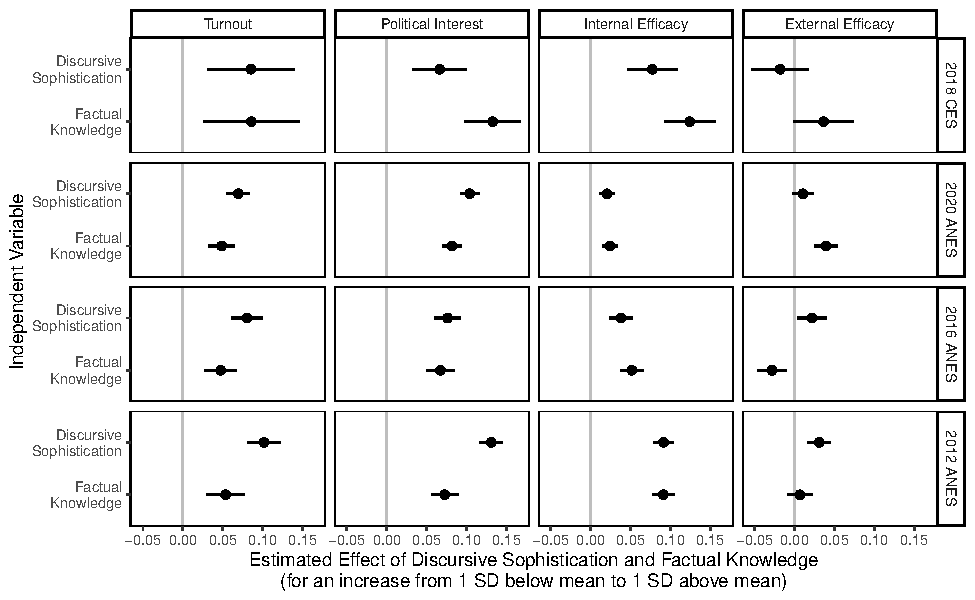
\includegraphics{/data/Dropbox/Uni/projects/2016/knowledge/fig/knoweff.pdf}
\caption[Effects of sophistication on turnout, political interest, internal efficacy, and external efficacy]{Effects of sophistication on turnout, political interest, internal efficacy, and external efficacy in the CES and ANES. For each dependent variable, the figure displays the average marginal effects (AME) for each sophistication measure (including 95\% confidence intervals). Model estimates are based on logistic regression (turnout) or OLS (political interest, internal efficacy, external efficacy). Each analysis includes controls for gender, education, income, age, race, and church attendance. Full model results are displayed in the appendix, Tables~\ref{tab:knoweff2018cces} through \ref{tab:knoweff2012anes}.}\label{fig:knoweff}
\end{figure}

Each panel compares the average marginal effects of both sophistication measures on the respective dependent variable while holding all other variables constant at their means. Of course, these effects are purely correlational and should not be interpreted causally. Nevertheless, across all four surveys, discursive sophistication is a stronger predictor of turnout, political interest, and internal efficacy. The results for external efficacy are more ambiguous. Factual knowledge has strikingly inconsistent effects---sometimes predicting higher, lower, or no change in external efficacy. Discursive sophistication, in contrast, is more consistently associated with higher external efficacy (the only exception is the 2018 CES, which uses a shorter battery to measure external efficacy).

Considering these initial results, a potential concern may be that discursive sophistication is confounded by individual characteristics that influence verbatim response patterns as well as engagement. Appendix~\ref{app:personality} provides additional analyses controlling for factors that might drive verbosity such as personality (extraversion), survey mode (face-to-face vs. online), verbal skills, as well as individual response length itself. The substantive conclusions remain unchanged.


\subsubsection*{Incorporation of New Information}
In order to replicate and extend this first validation, I rely on a separate nationally representative survey employing an alternative set of open-ended responses. The data was collected by YouGov in December 2015 and contains responses of 1000 U.S. citizens. %\footnote{See \citet{clifford2018disgust} for details on the study.} 
% TODO: add footnote again after reviews
As part of this study, respondents were asked four open-ended questions to describe their attitudes towards two salient issues: gun legislation and the Affordable Care Act.

% TODO: add arguments regarding procedural knowledge here

Political sophistication should imply the ability to incorporate relevant new information about parties, office-holders, and policies. After all,  \citet{zaller1990political,zaller1992nature} and others argue that tests of factual information about politics are the best available proxy for awareness. In this analysis, I explore whether discursive sophistication or factual knowledge serves as a better predictor of people's ability to incorporate new information from media sources. As part of the survey, respondents were asked to read a newspaper article about a fictional infectious disease and were subsequently asked to answer questions about information provided in the article (e.g. regarding symptoms, modes of contraction etc.). I compute an additive index counting the pieces of information that were correctly recalled (\textit{information retrieval}) as a measure of the ability to retrieve information from a news article on a non-partisan issue that is related to public health policies. 

\begin{figure}[h]\centering
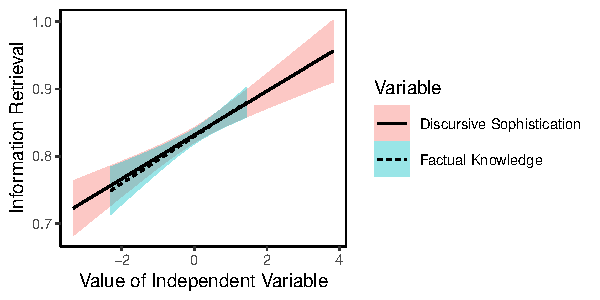
\includegraphics{/data/Dropbox/Uni/projects/2016/knowledge/fig/yg_disease.pdf}
\caption[Expected information retrieval in the 2015 YouGov Study as a function of political sophistication]{Expected information retrieval in the 2015 YouGov Study as a function of political sophistication (including 95\% confidence intervals). Estimates are based on a linear regression model controlling for education, income, age, church attendance, gender, and race. Full model results are displayed in the appendix, Table~\ref{tab:yg_disease}.}\label{fig:yg_disease}
\end{figure}

Figure~\ref{fig:yg_disease} displays the relationship between political sophistication and disease information retrieval in the 2015 YouGov study. Estimates are based on linear regression models controlling for education, income, age, church attendance, gender, and race. As a benchmark for discursive sophistication, I again consider the effect of factual knowledge based on a battery of eight items similar to the knowledge questions in the ANES. Both discursive sophistication as well as factual knowledge increase the amount of information individuals are able to recall from a news article discussing a fictional disease. Similar to the previous results, the effects are stronger for discursive sophistication than for factual knowledge scores. The degree to which citizens discuss their own political beliefs in a more elaborate manner is not only a stronger predictor of political engagement but also serves as a better proxy for the ability to incorporate new information about a non-partisan issue.


\subsubsection*{Well-Justified Policy Preferences}
As the last validation step, I examine an additional set of surveys that provide a unique opportunity to compare my proposed measure of discursive sophistication with manually coded open-ended responses across three languages.  \citet{colombo2016justifications} compiled a data set of cross-sectional surveys administered in Switzerland after national popular votes on multiple policy propositions. For each referendum, respondents were asked to explain why they voted in favor or against a given proposition in two separate open-ended items. Based on these verbatim responses, I computed the discursive sophistication using the same procedure outlined above. Since the survey was conducted in three different languages (German, French, and Italian), I created separate metrics for each group of respondents.

Beyond the ability to incorporate new information, political sophistication should enable people to justify their own preferences. Colombo's \citeyearpar{colombo2016justifications} manual coding of the respondents' \textit{level of justification} assessed the content, elaboration, and complexity of open-ended responses. Thus, this study provides an opportunity to directly assess the extent to which high levels of discursive sophistication correspond to well-justified policy preferences in open-ended responses. Any overlap between Colombo's \citeyearpar{colombo2016justifications} manual coding with my automated measure corroborates the face validity of discursive sophistication.

The results are presented in Figure~\ref{fig:swiss_ggridges}, which displays the distribution of discursive sophistication for each level of justification coded by \citet{colombo2016justifications} as well as the correlation coefficients for both respective variables. Across all three language groups, discursive sophistication is systematically higher among respondents with the highest level of justification and both measures are positively correlated ($r=0.23, 0.32$, and $0.36$). The proposed measure of discursive sophistication therefore shows a high degree of correspondence with individual levels of justification assessed by independent manual coders.

\begin{figure}[h]\centering
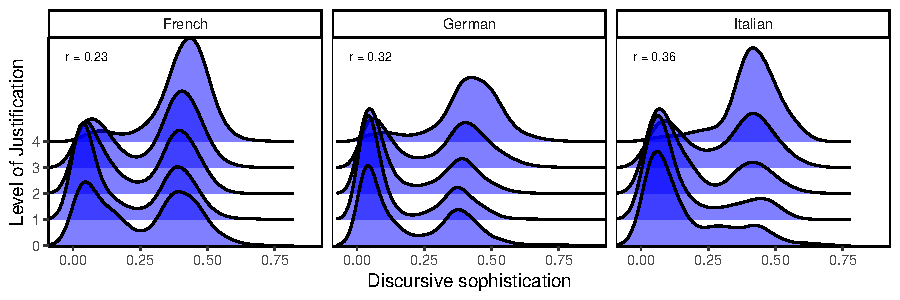
\includegraphics[scale=1]{/data/Dropbox/Uni/projects/2016/knowledge/fig/swiss_ggridges.pdf}
\caption[Discursive sophistication and manually coded level of justification in Swiss post-referendum surveys]{Discursive sophistication and manually coded level of justification \citep{colombo2016justifications} in Swiss post-referendum surveys. The plot compares kernel densities of discursive sophistication for each manually coded level of justification.}\label{fig:swiss_ggridges}
\end{figure}

To summarize, the results presented thus far indicate that discursive sophistication shares common characteristics with factual political knowledge measures. At the same time, the proposed measure outperforms conventional metrics as a predictor of political participation and engagement, provides a better proxy for the ability to incorporate new information from news sources, and shares significant overlap with manually coded levels of justification in open-ended responses. Next, I illustrate how discursive sophistication can help refine previous findings regarding the gender gap in political knowledge.

%\clearpage
\subsection*{Reassessing the Gender Gap}
How do women and men compare on the different metrics of political sophistication in the surveys analyzed in the present study? Figure~\ref{fig:meandiff} displays the average levels of discursive sophistication and conventional metrics comparing both genders. While we observe a sizable and statistically significant gender gap for factual knowledge across the CES, ANES, and YouGov surveys, this difference disappears for discursive sophistication. Even though women do not perform as well as men on political quizzes, they do not differ substantially in complexity and sophistication when describing their political preferences.

\begin{figure}[ht]\centering
	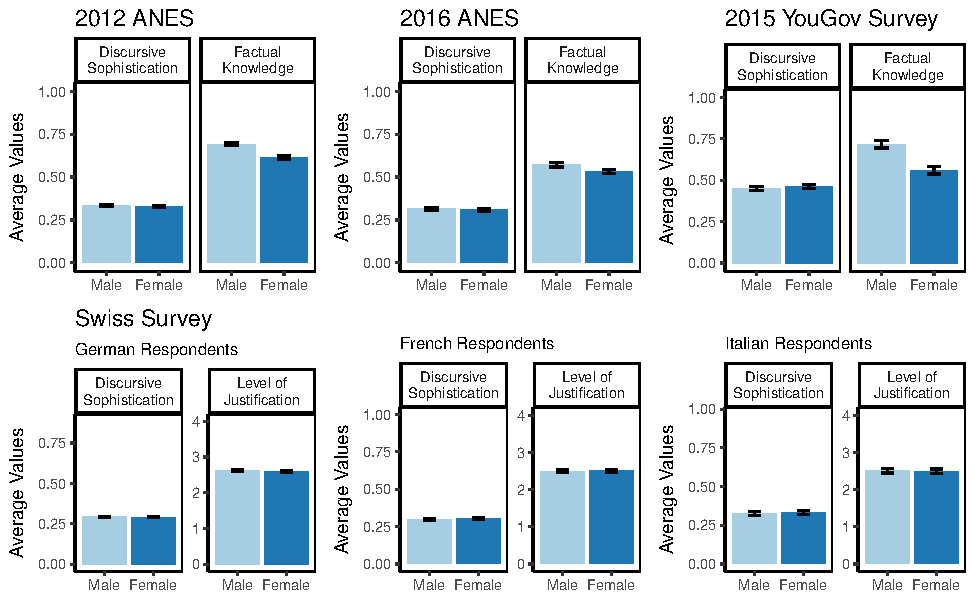
\includegraphics[scale=1]{/data/Dropbox/Uni/projects/2016/knowledge/fig/meandiff.pdf}
	\caption[The gender gap in political sophistication]{The gender gap in political sophistication. The figures display mean levels of discursive sophistication (light blue) and factual knowledge (dark blue) comparing women and men (including 95\% confidence intervals). All gender differences in factual knowledge are statistically significant with $p<.05$.}\label{fig:meandiff}
\end{figure}

%\clearpage

Of course, we need to make sure that this absence of a gender gap in discursive sophistication is not idiosyncratic to the particular measurement approach proposed here. One way to investigate this question is to examine gender differences in discursive sophistication using data from \citet{colombo2016justifications} and comparing them to her manually coded measure. That way, we can not only determine whether the lack of a gender gap in discursive sophistication replicates in the Swiss survey, but also check whether there is an equivalent lack of gender differences in Colombo's alternative measure of citizen competence in direct democracies. If discursive sophistication captures a person's motivation to undertake in-depth reasoning and form quality opinions (and assuming these characteristics do not differ by gender), there should be no difference between women and men on either metric (discursive sophistication and Colombo's measure). As shown in the bottom row of Figure~\ref{fig:meandiff} there are indeed no significant gender differences on \textit{both} metrics across all three languages in the Swiss referendum surveys. The absence of a gender gap is consistent whether open-ended responses are coded manually or using the proposed measure of discursive sophistication.

Next, we have to consider whether the apparent gender gap in factual knowledge is a manifestation of real differences between women and men. Prior research attributes at least part of the gap to actual discrepancies in individual resources and engagement. Accordingly, we need to control for these determinants of political knowledge to provide a more comprehensive examination of the veracity of observed gender differences. Figure~\ref{fig:determinants} displays estimated gender differences after controlling for various potential common determinants such as education, income, age, race and church attendance.

\begin{figure}[h]\centering
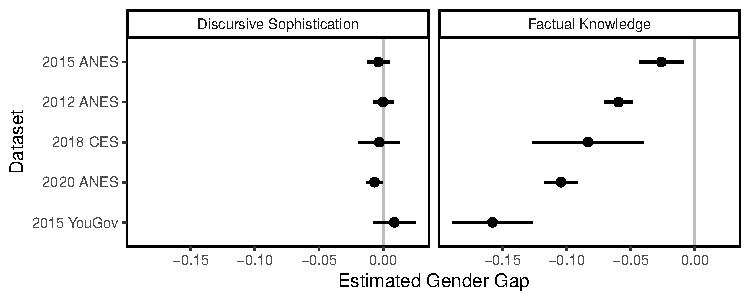
\includegraphics{/data/Dropbox/Uni/projects/2016/knowledge/fig/determinants.pdf}
\caption[The gender gap in political sophistication after controlling for common determinants.]{The gender gap in political sophistication controlling for common determinants. Estimates are OLS regression coefficients with 95\% confidence intervals. Dependent variables are discursive sophistication and factual political knowledge. Estimates are based on a linear regression model controlling for education, income, age, church attendance, gender, and race. Full model results are displayed in the appendix, Tables~\ref{tab:determinants_text} and \ref{tab:determinants_factual}.}\label{fig:determinants}
\end{figure}

After controlling for common determinants, discursive sophistication again reveals no significant differences between women and men across the CES, ANES and YouGov surveys.\footnote{I did not include the Swiss study in this comparison because the survey did not include comparable factual knowledge items. Suffice to say that there are no significant gender differences in discursive sophistication in the Swiss study when including sociodemographic cotrols.} The gender gap in factual political knowledge, however, persists and is substantively as well as statistically significant. Thus, a considerable portion of the observed differences in factual knowledge between women and men cannot attributed to underlying disparities in resource-related factors or engagement. Comparing the confidence intervals across both measures further reveals that the insignificant gender differences in discursive sophistication are estimated with higher precision than the significant differences in factual knowledge. Such a result precludes the possibility that null findings for discursive sophistication are purely driven by measurement error on the dependent variable. It is also worth pointing out in this context that the effects of control variables are quite similar across both measures and different surveys.\footnote{See Appendix~\ref{app:tables} for full regression results.} For instance, knowledge and discursive sophistication are significantly higher among respondents who are more educated and have higher income. The finding that determinants of political sophistication are consistent across models lends additional validity to the open-ended measure.%\footnote{An interesting deviation, however, is the effect of survey mode in the 2012 and 2016 ANES. Respondents in online surveys score significantly higher on factual knowledge than in face-to-face interviews. This difference can be attributed to the fact that individuals are able to look up answers for factual knowledge questions while taking an online survey \citep[cf.][]{clifford2016cheating}. For discursive sophistication, on the other hand, individuals perform better in the face-to-face survey. Open-ended answers in online surveys may be less elaborate because respondents have to manually type their responses.} % NOT CONTROLLING FOR MODE HERE!

% TODO: One could argue (see R3) that this lack of gender differences is due to higher measurement error in discursive sophistication. This is unlikely to be the case since other common predictors of discursive sophistication have a similar size / magnitude as the factual knowledge model. See table in Appendix for more information.


\subsection*{Explaining the (Lack of a) Gender Gap}

% Summarizing the results thus far, there is no evidence for systematic differences between women and men in discursive sophistication.
To summarize, conventional knowledge measures and discursive sophistication produce diverging conclusions regarding the existence of a gender gap. This naturally raises the question which metric we should ultimately trust? Prior research attributed gender differences in factual knowledge---at least partly---to the format (e.g., availability of ``Don't Know'' options) and content (e.g., focusing on issues that are less relevant to women) of item batteries. This section explores whether these arguments provide a sufficient explanation for the conflicting results for discursive sophistication---namely the complete lack of systematic differences between women and men. In other words, which one is more likely to be an artifact of the respective measurement approach: the \textit{existence} of a gender gap in factual knowledge or the \textit{absence} of a gap in discursive sophistication?

The first set of arguments about why conventional metrics may overstate potential gender differences is based on the finding that women are less likely to guess than men \citep{mondak2004knowledge}. Arguably, respondents' differential willingness to admit not knowing the answer to a question is certainly less of an issue when they are simply asked to voice their opinions rather than being quizzed on political facts. Following best practices, however, the surveys presented here omitted ``Don't Know'' options in their recall questions. Differential propensity to guess can therefore not be viewed as a valid explanation for the gender gap in factual knowledge observed here. At the same time, the lack of significant differences between women and men in discursive sophistication may itself be the product of selection biases in women's willingness to answer open-ended question in the first place. Following this argument, it could be the case that only women who are highly sophisticated provide a response, thereby misleadingly closing the gender gap in the discursive measure. There are two reasons why that is unlikely to be the case. First, as the analyses have shown, this proposed selection mechanism does not diminish gender differences in factual knowledge. Second, and more importantly, there are no significant differences between men's and women's willingness to answer open-ended questions. In fact, adjusting for potential selection effects when examining determinants of sophistication does not change the substantive conclusions.

% TODO: clarify this section and discuss issue of DK in OE responses -> no gender diff!

The second major explanation for the gender gap in political knowledge focuses on the question content. By choosing a specific set of recall questions as a general metric for political knowledge, researchers are making strong assumptions about the information deemed necessary for competent decision-making. As it turns out, these item batteries usually focus on male-dominated topics in politics \citep{dolan2011women}. Open-ended questions, on the other hand, make it possible to directly study the information that is in fact available to citizens and---importantly---to examine how they apply their knowledge when discussing their political preferences.

Accordingly, if it is the case that the gender gap in discursive sophistication is nonexistent simply because open-ended questions allow women to raise political considerations particularly salient to them, then we should be able to observe systematic variation in types of issues discussed by women and men, respectively. Luckily, we can directly examine such gender differences in topic prevalence within the structural topic model framework used to measure discursive sophistication. More specifically, gender is included in the model as one of the covariates that influences how often each topic is discussed by a respondent \citep[see also][for details]{roberts2014structural}.

\begin{figure}[ht]\centering
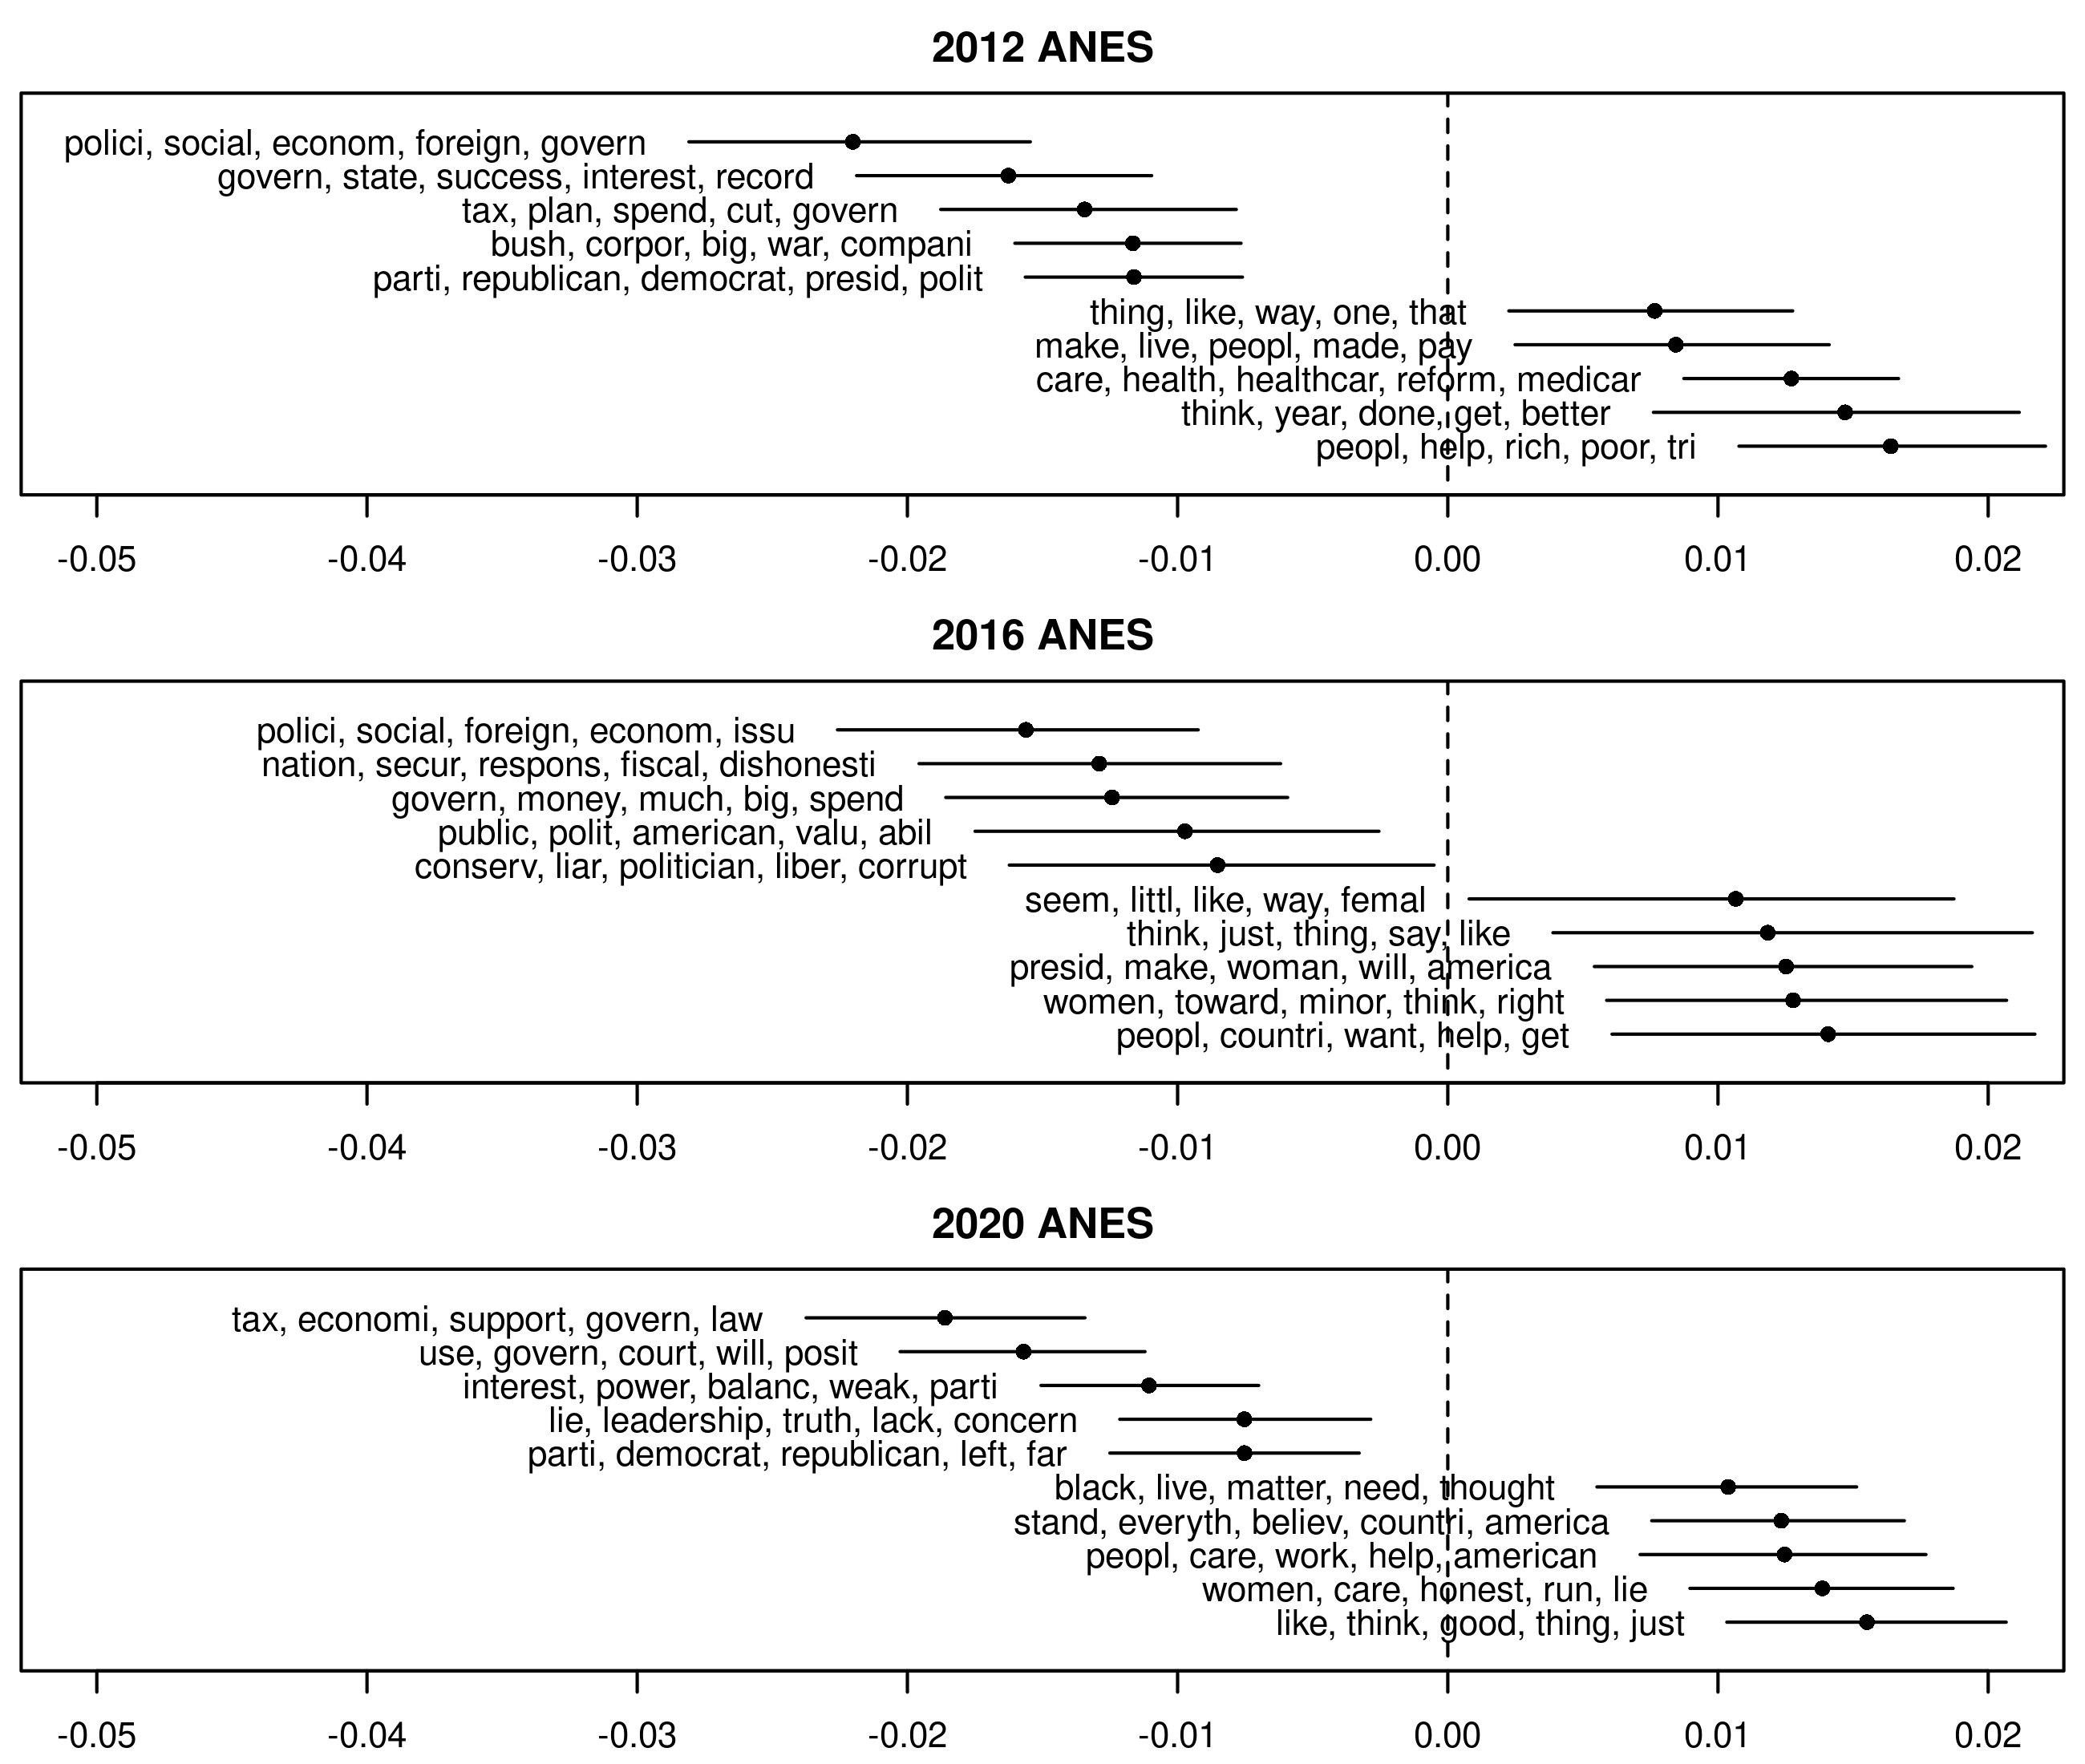
\includegraphics[width=.9\textwidth]{/data/Dropbox/Uni/projects/2016/knowledge/fig/stm_gender.png}
\caption[Gender differences in topic proprtions in open-ended responses]{Gender differences in topic proportions in open-ended responses based on the structural topic model used to compute discursive sophistication (including 95\% confidence intervals). Coefficients indicate the difference in predicted topic prevalence among women and men; positive values indicate higher prevalence among women. Labels are based on the five highest probability terms related to the topic.
%Full model results are displayed in the appendix, Table~\ref{tab:determinants}
}\label{fig:stm_gender}
\end{figure}

In this last analysis, I therefore explore how women and men differ in topical prevalence across open-ended responses in the 2012, 2016, and 2020 ANES. Note that these open-ended items did not focus on specific issue areas as in the CES, but rather asked respondents to evaluate different political parties and candidates. Thus, they were able to focus on whatever issue they deemed most important. Figure~\ref{fig:stm_gender} displays the subset of topics that shows the largest absolute gender difference in topic prevalence in both waves. Positive coefficients indicate that women are more likely than men to mention a given topic, and vice versa. The top five topics are more prevalent among men and the bottom five are more likely to be mentioned by women. The label for each coefficient consists of the five highest probability terms related to the topic to illustrate its content.

Taking the 2012 ANES as an example, the topic consisting of terms such as \textit{care}, \textit{health}, and \textit{reform} is significantly more likely to be mentioned by women. On the other hand, men are more likely to mention the topic revolving around terms like \textit{tax}, \textit{spend}, and \textit{cut}. Overall, across both waves of the ANES, women were less likely than men to discuss foreign affairs, economic issues, or the Supreme Court. Instead, they focused on issues related to women's rights, equality, and health care. The considerations raised by women when discussing their political preferences are therefore clearly different from men's and---crucially---the issues discussed by men happen to be more aligned with the type of questions usually covered in standard political knowledge batteries (i.e., pertaining to the economy, institutions, elites, etc.). For example, men are more likely to mention considerations related to the federal budget in their open-ended responses. At the same time, two of the five knowledge questions included in the 2012 ANES pertain to government spending: one asking respondents to compare the federal deficit to levels in 1990, the other requiring a comparison of federal spending on different programs such as foreign aid, medicare, and national defense.

Overall, the results indicate that gender differences in conventional knowledge metrics are at least partly driven by the fact that the issues women care about are not represented in standard item batteries. When using the alternative measure---discursive sophistication---any evidence for systematic differences between women and men disappears since open-ended questions about political preferences allow respondents to focus on different issues. 

% TODO: Make a connection back to Druckman here?


\section*{Discussion}
% What is a competent citizen? One who has good reasons for his or her attitudes... we can measure that when examining how repondents talk about their political beliefs.

% 3) Discuss implications for competence and tie back to Druckman's argument
From a normative perspective, there is no reason to assume that a particular set of issues should be more important for citizens' preference formation or competence in elections. Whether one cares more about the federal budget or reproductive rights, the most important question is whether citizens think deeply about the issues they care about and incorporate them accordingly when making their vote choices. As \citet{druckman2014pathologies} argues, citizen competence (for example in elections) should not be evaluated based on their ability to recall unrelated facts about political institutions, but rather focus people's motivation to form quality opinions---which implies that they focus on the issues most important to them. As it turns out, while the types of issues raised women and men differ systematically, there is no reason to assume that women are therefore less sophisticated or competent in the realm of politics.

% 4) Discuss how discursive sophistication can be used to improve knowledge batteries
This issue has been recognized in the literature before \citep[e.g.,][]{graber2001processing,dolan2011women,ferrin2020gender}, but it cannot be properly addressed while relying exclusively on off-the-shelf recall questions to measure political knowledge. What is more, there is thus far no principled approach to develop new sets of items that focus less on male-dominated issues. Beyond proposing an alternative measurement approach, the framework presented in this paper can help provide such a first step towards devising balanced recall items. More specifically, examining the types of issues women and men emphasize when discussing their political preferences can serve as a guide to select new sets of knowledge questions. Thus, future research should explore whether factual knowledge questions selected based on open-ended responses are indeed more balanced with regard to gender differences. To the extent that this proves to be a useful heuristic for item selection, researchers planning a survey could rely on pilot studies fielding open-ended questions in order to devise balanced factual knowledge items in the main survey.

% 5) Mention potential drawbacks and disadvantages
That being said, relying on open-ended responses to assess political sophistication has its limitations. First and foremost, elaboration in verbatim attitude expression may be more prone to biases due to differential levels of motivation to answer survey questions. It should be noted, however, that conventional knowledge metrics are not free from survey effort effects either---as indicated for example by the fact that scores can be improved by providing monetary incentives for correct responses \citep{prior2008money}---and future studies should investigate the extent to which discursive sophistication is subject to similar deviations. A related potential confounding factor that is unique to open-ended responses is the respondents' general linguistic skills or verbal verbosity, which may again influence elaboration in open-ended responses but is orthogonal to political sophistication.

% 6) Discuss why the issues are probably not that bad
One reason why these potential drawbacks may be less worrisome is that the proportion of respondents who refuse to answer any open-ended question in the first place is very low, which indicates that people are sufficiently motivated to engage with the survey. Furthermore, controlling for pure response length did not change the substantive conclusions regarding the effects of discursive sophistication on, for example, political participation or efficacy. The results were also robust to the inclusion of measures of linguistic skills or personality characteristics such as extraversion. In a similar vein, the gender gap finding did not appear to be driven by selection effects, which again suggests that survey effort---albeit an important confounding factor to consider---is unlikely to jeopardize the substantive conclusions presented in this paper.

% 7) Bring up survey mode, discuss advantage regarding cheating
% Nevertheless, it is important to keep in mind the differential role of survey mode when comparing factual knowledge and discursive sophistication. Open-ended responses in face-to-face or phone interviews are relatively effortless since they are not unlike voicing your opinion in regular conversations and do not require respondents to transform their thoughts into fixed response categories \citep[e.g.,][]{sudman1996thinking}. Unsurprisingly though, respondents tend to provide less elaborate responses in online surveys, resulting in systematically lower discursive sophistication scores (see Figure~\ref{fig:determinants}). Knowledge quizzes conducted online, on the other hand, are prone to bias in the opposite direction due to respondents' tendency to cheat by looking up correct answers \citep{clifford2016cheating}. Ultimately, more work is needed to explore how survey mode affects discursive sophistication and factual knowledge scores, especially focusing on ways to reduce the effort in answering open-ended questions in online surveys.

% 8) Manual coding as an alternative to overcome these issues?
Lastly, even if one supports the general notion that open-ended responses can provide useful insights, a skeptic may still argue that manual coding is preferable to the automated framework presented here. However, manual coding of open-ended responses is not always feasible in the context of large-scale surveys, since it can be labor-intensive and requires extensive contextual knowledge such as high levels of language proficiency. The Swiss surveys in Colombo's \citeyearpar{colombo2016justifications} study, for example, were conducted in three different languages (German, French, and Italian) and ranged across numerous policy referenda. More importantly, knowledge assessments can be biased by the level of political agreement between individuals \citep[e.g.,][]{ryan2011accuracy}. The measurement approach presented here, on the other hand, is easily replicable and reproducible, is not affected by subjective judgments, and can be directly applied to large-scale surveys in multiple contexts across different languages.

\section*{Conclusion}

% 1) Repeat general argument
Political scientists should worry less about pure levels of \textit{factual knowledge} and instead focus on how people justify their political preferences. Factual knowledge about political institutions might be a useful proxy in certain scenarios, but it cannot address directly whether individuals hold well-considered opinions about political actors or issues. In comparison, the measure of discursive sophistication proposed here is agnostic about the specific contents of people's beliefs, but directly targets the complexity of expressed attitudes. It can therefore be easily applied to assess sophistication in any decision-making context (such as policy referenda or local elections) by fielding targeted open-ended questions related to the relevant underlying beliefs and preferences. Furthermore, a free software package for the statistical programming environment R will allow applied researchers to implement the framework presented here.\footnote{Package under development, release on CRAN expected mid 2022.}

% 2) Summarize main findings of the paper
The findings presented in this paper show that conventional knowledge indices and the open-ended measure share a substantial amount of variance. However, they are far from being identical and capture different aspects of sophistication. In fact, discursive sophistication is a stronger predictor of political engagement and efficacy than traditional metrics. It is also strongly related to people's ability to incorporate new information from news sources and shows a high degree of overlap with manually coded levels of justification. Most importantly, using the discursive measure, any evidence for the gender gap commonly reported using factual knowledge scales disappears. Women might know fewer facts about political institutions, but they do not differ substantively in the complexity of their expressed political beliefs. Furthermore, the lack of gender differences in discursive sophistication can be attributed to the fact that open-ended questions allow women to focus on different considerations than men.

% 9) BIG CONCLUSION: clearly state that it is not to be viewed as a replacement but rather a substitute for political knowledge questions
In the past, scholars have argued that testing for factual information, despite its shortcomings, still provides the best available measure of political awareness as it captures ``what has actually gotten into people's minds, which, in turn, is critical for intellectual engagement with politics'' \citet[21]{zaller1992nature}. The results presented in this paper suggest that a direct examination of open-ended responses provides a viable supplemental approach that promises new insights into how people make up their mind about politics.

